\chapter{Design and Implementation} \label{chap:impl}

We have built a system (shown in Fig \ref{fig:overview}) that is able to generate metabolic models of cell-free systems.
Our system takes in cell-free experimental data, converts it into a metabolic model, and then performs dimensionality reduction to reflect the experimental data.

\section{Data gathering}
In order to build a robust model that reflected biological reality, we first had to generate the data we wanted to use for training.
Gathering high quality biological data is difficult and was a crucial key to the success of the system as a whole.
We describe the high level process of creating a cell-free system and running the experiments below, while the full protocol can be found in the Appendix.

\subsection{Cell-free systems}
As shown in Fig \ref{fig:cfps}, creating a cell-free protein expression system involves three main steps: growing and lysing cells, supplementing with energy substrates, and adding custom DNA constructs.
Our protocol is based off of the open protocol out of the Federici lab \cite{medina2017cfps}.
We begin by growing up 1L of BL21 E. coli cells in an overnight culture of LB until they have reached OD of 1.6.
Then, we spin down the cells and remove the supernatant, storing the pellet in the refrigerator overnight if necessary.
Next, we perform 3 more sets of spins and washes with S30 buffers to remove any extracellular debris.
Finally, we use a bead beater to lyse the cells and spin one last time to remove the cellular debris and beads.
At the end of this process we have cell extract which can be stored in a -80\degree freezer.
See Appendix \ref{app:exp} for the full detailed protocol.

\begin{figure}[t!]
\begin{center}
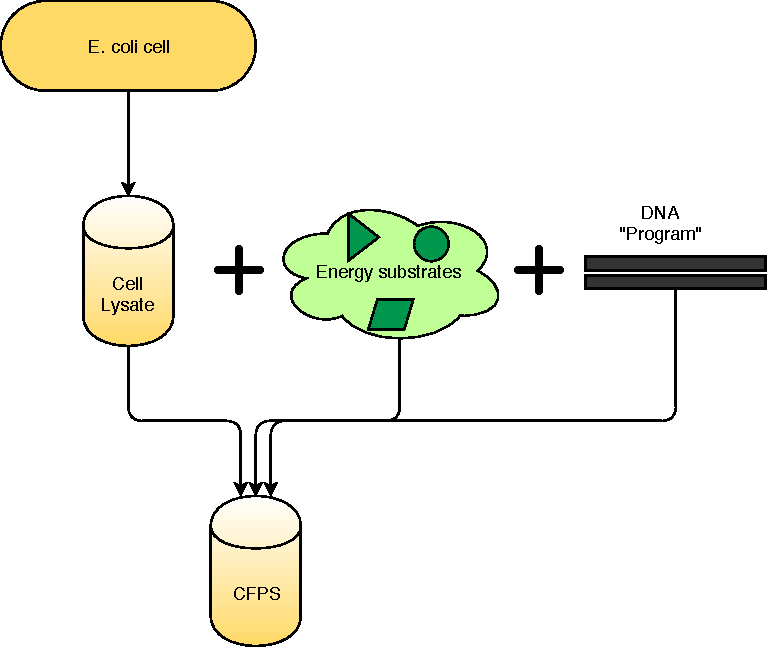
\includegraphics{figs/CellFreeSetup.pdf}
\caption{Overall process for creating a CFPS}
\end{center}
\label{fig:cfps}
\end{figure}

Once we have this cell extract, we have the core cellular machinery that is necessary for transcription and translation.
However, we need to add the cofactors and reactants that are important for the transcription and translation reactions.
So, we add energy substrates to the cell extract to create a cell-free protein expression system.
These substrates include energy substrates such as cAMP, maltodextrin, and NAD.
They also include vital parts of transcription and translation such as NTPs, AAs, and tRNAs.
See Table \ref{tab:cf-nrg} for a complete listing of the reactants and the concentrations we use.

\begin{table}[]
\centering
\caption{List of reactants for a 50 $\mu L$ CFPS reaction. 
Note that MDX is a mixture of substrates and that AAs include all 20 of the amino acids.}
\label{tab:cf-nrg}
\begin{tabular}{lll}
Reactant     & Amount ($\mu L$) & Purpose                         \\
MDX          & 5               & Energy substrates               \\
AAs          & 10              & Building blocks for translation \\
PEG          & 2.5             & Molecular crowding              \\
HMP          & 1               & Phosphate source                \\
Mg           & 0.74            & Important cofactor              \\
K            & 0.8             & Charge homeostasis              \\
Cell Extract & 25              & TX/TL machinery                 \\ \hline
CFPS         & 50              & Protein production             
\end{tabular}
\end{table}

Given this cell-free expression system, we have essentially assembled a biological computer.
Whatever DNA "program" is added, the system will work to produce the appropriate protein result.
This platform is incredibly powerful because it allows us to easily insert these DNA programs and see results within a few hours.
A typical biological timeline would take far longer because living cells would have to be coerced to uptake the DNA and incorporate it into their production process.

\begin{table}[]
\centering
\caption{My caption}
\label{tab:cf-conc}
\begin{tabular}{ll}
Compound     & Concentration (mM) \\
pi           & 0.981              \\
mg           & 5.92               \\
k            & 48.0               \\
nad          & 0.454              \\
coa          & 0.353              \\
camp         & 1.01               \\
folinic acid & 0.092              \\
spermidine   & 0.181              \\
glucose      & 5.42               \\
ATP/GTP      & 2.09               \\
CTP/UTP      & 1.26               \\
amino acids  & 35.6               \\
trna         & 0.010              \\
dna          & 0.071             
\end{tabular}
\end{table}

%TODO talk about debugging/contamination issue

\subsecton{Datasets}
Once that protocol was established and standardized as a reliable means of protein production, we were able to create two datasets.
Our first dataset followed the typical procedure a biologist in the lab would use to create a CFPS.
We combined each of the ingredients by hand into a 50 uL mastermix and then used 5 uL aliquots of that for our test conditions.
In order to test different reaction conditions, we added an additional 1 uL of sugar, phosphate, or nucleotides in differing ratios.
These different ratios of additional reactants are our independent variables.
Since we added just a simple DNA circuit that produces RFP, the fluorescence readout is our dependent variable.

However, there are multiple downsides to doing this by hand.
First of all, it takes a long time and so there is a limit to the amount of data one can generate.
Additionally, pipetting by hand has an intrinsic error.
To get around these issues, we also generated a larger dataset using the Labcyte Echo robot.
This is an acoustic liquid handler that allowed us to generate a dataset in the same spirit as before, though we were able to vary a much larger array of reactions conditions and perform the experiments at the 2 uL volume.

Finally, we received a third dataset from the recent Karim and Jewett paper \cite{karim2018controlling}.
Our protocol is based off of the CFPS from the Jewett lab, so it is a very similar setup.
However, it was created in different lab conditions, so we can check to see if our model generalizes across lab conditions.
Additionally, the pathway that they investigated is an inherently metabolic pathway, so we were able to easily incorporate it into our metabolic model.

\section{Data ingestion and incorporation}
Since this system is intended to aid biologists in their experiments, we wanted to make it end-to-end and as easy to use as possible.
With that in mind, we created tools to automatically incorporate the experimental setup into the models.
There are two main ways that the experimental setup could show up.
The first is in the form of end concentrations of the different reactants in the cell-free system.
This is the easiest because we are able to convert concentrations into fluxes.
Thus, our tool is able to ingest that in the form of a CSV that has a column with the name of the reactant and the final concentration.

However, we also support biologists who just know the relative amounts of each reactant they add to the mixture without knowing the final concentration.
Thus, we support a format whereby a user can upload a CSV that contains the name of each reactant, the molecular weight, the volume used to create the stock, the weight used to create the stock, and the final volume added to the cell-free reaction.
From that, we are able to calculate the final concentrations and manipulate the data into the same form as the first type of upload.
Once we have that, we can unify the pipeline.

\begin{figure}[t!]
\begin{center}
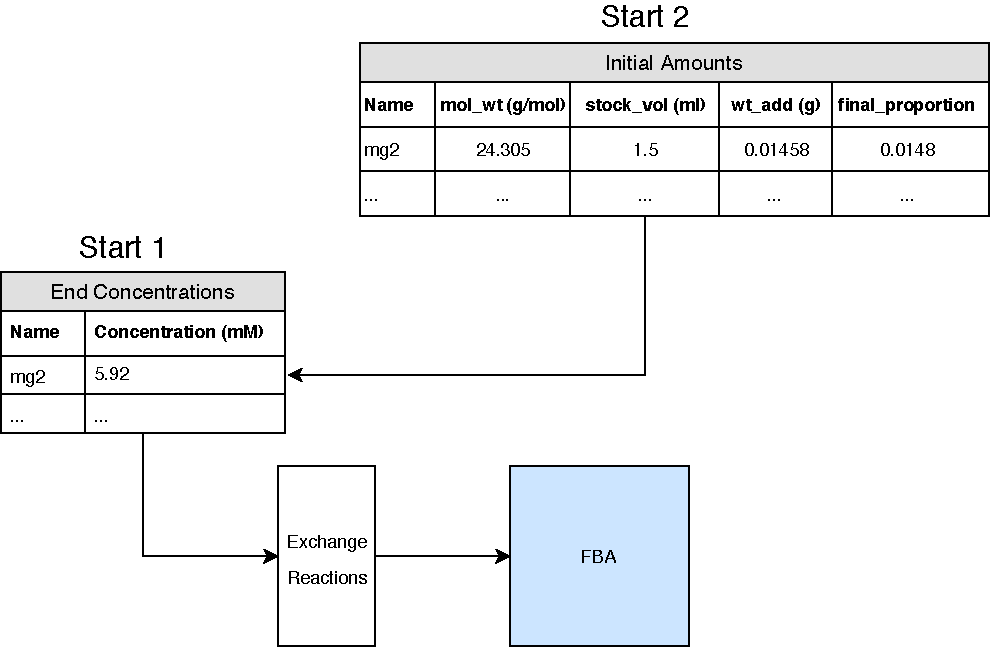
\includegraphics{figs/DataIngestion.pdf}
\caption{}
\end{center}
\label{fig:ingest}
\end{figure}


2 csvs
1 for experimental setup
2 columns, one with canonical abbreviation of chemical, other with end concentration
This data then gets converted into fluxes and put in as a constraining exchange reaction

Use Varner model and put gene sequence in file
Gene sequence automatically converted to appropriate NTP and AA numbers in varner model
Varner model then converted to python
TXTL reactions extracted and objective set as protein output.

1 for experimental results
columns are different reactants
rows are different starting conditions
last row is output (fluorescence or HPLC)

\section{FBA and flux sampling}

\subsection{FBA}

Were we simply to solve the different models we've created, many would have the same flux results.
Bijective function which compresses the projection
Clearly, the FBA doesn't describe the full richness of a real system
Need to do better with dimensionality reduction

Also have the problem that it's overspecified
These FBA models contain every reaction that's occurring in a steady state bacterium
While we do harvest the bacteria at this timepoint, not every reaction is going to maintain its importance
Can't encapsulate this solely in a change of objectives

If we just run the naive FBA models on the different reaction conditions, we find that we have a correlation of almost 0.
This means that the typical FBA model just doesn't describe CFPS
So, we want to use a VAE to improve the way we describe CFPS.
However, we first need a large dataset to train on.
The way we accomplish this is by flux sampling from each model.

\subsection{Flux sampling}
In order to determine possible fluxes through each reaction, need to sample from it
OptGP sampler
Can see that increasing the number of samples leads to a more normal distribution
Fig \ref{fig:fl-samps}

We sample from our different reactions to generate a new dataset.
Each experimental condition has slightly different flux distributions for each reaction.
This is important because it's these minor perturbation that we hope to use to create a specified model.

\section{VAE}
We implemented a VAE in order to examine the latent space of the 
Our original implementation simply took in the flux dataset as a $n x D$ matrix X with a vector $n x 1$ y that specified the "class" of each flux (i.e. which model it came from).
We then ran it through a 2 layer autoencoder with layer sizes TODO and TODO.
We experimented with latent dimensions of size 2 and 10.
This created a latent space of size $n x 2$.

We were able to explore this latent space.
However, this only reflects information about the fluxes.
We wanted to incorporate the experimental data we'd gathered--we know which models should be producing more fluxes than the others.
We used this insight to create a new loss function for our autoencoder.

\section{Correlated VAEs}
We have additional information that we can use to perturb our latent space.
We know what the relative rankings of the different models should be.
So, instead of just having the typical loss function of an autoencoder: reconstruction loss and KL divergence, we add another term that we call correlation loss.
We are forced to use pearson correlation loss because we can write that in a differentiable manner.

\section{FBA model reduction}
Finally, now that we have run our models through the Corr-VAE and achieved a latent representation, we need to use the insights we've generated to create better models.
We can do this in two ways.
Firstly, we could do this by any time we want to generate new data, we first generate the FBA model using the tool chain described above.
Then, using the trained autoencoder, we can transform the optimal fluxes and get the shifted optimum and see if that still is better.
This could be very useful for batch variation.

However, it would also be nice to not have to run it through an autoencoder each time.
Instead, we could use the insights we've gained to actually create a more accurate reduced model.
We do this by thresholding the latent space and removing reactions that have fluxes similar to 0.
This allows us to create more useful reduced models.
Now, running these reduced models with the differential conditions gives us a correlation of up to 0.5.

\cite{ebrahim2013cobrapy}